%%%%%%%%%%%%%%%%%%%%%%%%%% lecture-9
\begin{frame}[shrink]
  \frametitle{lecture-9 主要内容}
  \framesubtitle{循环结构程序设计举例(续)}
  \tableofcontents[hideallsubsections]
\end{frame}

\section{循环结构程序设计举例(续)}

\begin{frame}[fragile]
附加题1: 求$s=a+aa+aaa+\cdots+a\cdots a$, 其中$a$是一个$1\sim 9$的数字。例如$a=2, n=4$时, $s=2+22+222+2222$, $a$和$n$由键盘输入。
\pause
\begin{columns}
\column{0.5\textwidth}
\begin{lstlisting}
int i,s,n,term = 0;
for(i=1,s=0; i<=n; i++) // 初始化循环变量用逗号隔开
{
   term = term*10 + a;
   s += term; 
}
\end{lstlisting}
\end{columns}
\end{frame}

\begin{frame}[fragile]
\small
附加题2: 韩信点兵。韩信有一队兵, 他想知道有多少人, 便让士兵排队报数:\\
按从1至5报数, 最末一个士兵报的数为1;\\
按从1至6报数, 最末一个士兵报的数为5;\\
按从1至7报数, 最末一个士兵报的数为4;\\
按从1至11报数,最末一个士兵报的数为10;\\ 
计算韩信至少有多少兵。 
\pause
\begin{columns}
\column{0.8\textwidth}
\begin{lstlisting}
int x=1;
for(;;x++)  // 循环体仅含if()结构,看作一条语句,'{}'可省略
    if(x%5==1 && x%6==5 && x%7==4 && x%11==10)
    { 
       printf("%d\n",x);  
       break;
    }
\end{lstlisting}
\end{columns}
\end{frame}

\begin{frame}[fragile]
附加题3-1: 求水仙花数。如果一个三位数的个位数、十位数和百位数的立方和等于该数自身,则称该数为水仙花数。 \\
编程求出所有的水仙花数。\\
~\\  
\pause
\begin{columns}
\column{0.6\textwidth}
解法一: 采用三重循环
\begin{lstlisting}
int i,j,k; // 百、十、个位
for(i=1;i<=9;i++)    // 百位
  for(j=0;j<=9;j++)  // 十位
    for(k=0;k<=9;k++)  // 个位
      if(i*100+j*10+k == i*i*i+j*j*j+k*k*k)  
        printf("%d\n",i*100+j*10+k);
\end{lstlisting}
\end{columns}
\end{frame}

\begin{frame}[fragile]
附加题3-2: 求水仙花数。如果一个三位数的个位数、十位数和百位数的立方和等于该数自身,则称该数为水仙花数。 \\
编程求出所有的水仙花数。\\
~\\ 
\pause
\begin{columns}
\column{0.6\textwidth}
解法二: 采用一重循环
\begin{lstlisting}
int m,i,j,k; 
for(m=100;m<=999;m++)
{
   i=m/100; j=m/10%10; k=m%10;  
   if(i*100+j*10+k == i*i*i+j*j*j+k*k*k)  
      printf("%d\n",i*100+j*10+k);
}
\end{lstlisting}
\end{columns}
~\\
\pause
\textcolor{blue}{思考: 输出共有多少个水仙数?}
\end{frame}

\begin{frame}[fragile]
附加题3-3: 求整数区间$[a,b]$中水仙花数的个数。
\pause
\begin{columns}
\column{0.8\textwidth}
\begin{lstlisting}
int n=0; //计数 
int a,b; // a,b 区间
int i,t;   // 循环变量,代表a,b区间的每个数
int sum; // i的各位立方和 
scanf("%d%d",&a,&b);
for(i=a;i<=b;i++) // 考察i是否水仙数
{  
  sum = 0; t=i; // 临时变量记住i; 易遗漏每次内层循环前sum要归0
  while(t!=0) // 累加各位立方 
  { sum+=pow(t%10,3); t=t/10; }
  if(sum==i) n++; // i是水仙数 
}
printf("%d\n",n);
\end{lstlisting}
\end{columns}
\end{frame}

\begin{frame}[fragile]
附加题4: 百钱百鸡, 已知公鸡5个钱1只, 母鸡3个钱1只, 小鸡1个钱3只, 用100个钱买了100只鸡。问公鸡、母鸡、小鸡各几只? 
\vspace{0.5cm}
\pause
\begin{columns}
%\column{0.9\textwidth}
\begin{lstlisting}
int x,y,z; // 公鸡、母鸡、小鸡个数
for(x=0;x<=100;x++) 
   for(y=0;y<=100;y++) 
     for(z=0;z<=100;z++) 
       if(5*x+3*y+z/3 == 100 && x+y+z == 100 && z%3 == 0) // 全部条件! 
          printf("%d,%d,%d\n",x,y,z);
\end{lstlisting}
\end{columns}
\vspace{0.5cm}
\pause
\textcolor{blue}{如何考虑无解的情况?}
\end{frame}

\begin{frame}[shrink,fragile]
附加题5-1: 求整数$a,b$的最大公约数,当两个数中有一个为0时,公约数是不为0的那个整数; 当两个整数互质时最大公约数为1。
输入两个整数a和b,求最大公约数。 
\pause
\begin{lstlisting}
#include <stdio.h>
int main()
{
  int a,b,t,i;
  scanf("%d%d",&a,&b); // 机试系统不要想当然给提示语句, 除非题目要求 
  if(a<b) { t=a; a=b; b=t; } // 交换a,b,使a是较大者 
  for(i=b;i>0;i--)
    if(a%i==0 && b%i==0){ t=i; break; } // 求得最大公约数 
  if(i==0)  // 如果循环结束,还未求得公约数,
  {
    if(b==0) t = a;
    else t=1; // a,b互质 
  } 
  printf("%d\n",t);
  return 0;
}
\end{lstlisting}
\end{frame}

\begin{frame}[shrink,fragile]{求整数$a,b$的最大公约数, 欧几里得算法}
\begin{columns}
	\column{0.6\textwidth}
	古希腊数学家欧几里德在其著作<<The Elements>>中最早描述了这种算法。\\
	\textbf{定理:}两个整数的最大公约数等于其中较小的那个数和两数相除余数的最大公约数。
	\column{0.3\textwidth}
	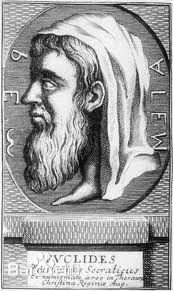
\includegraphics[scale=0.3]{eou}
\end{columns}
~\\
\textbf{伪代码分析}
\begin{lstlisting}
a,b的最大公约数,[则: a=mb+r, m=a/b; r=a%b]
循环, b作被除数,分母是余数r, 
[则: n=b/r; r=nb; a=mb+nb=(m+n)b; 如果一个整数能整除b, 必整除a]
直到r=0, 本轮循环的a(上轮循环的b)就是最大公约数。 
while(1)
{
   r = a%b; // 注意b为0时,不能计算余数,a就是最大公约数
   if(r==0) { gcd=a; break; } // 本轮循环的a(上轮循环的b)就是最大公约数
   a=b; b=r; // 准备下一轮迭代    
}
\end{lstlisting}
\end{frame}

\begin{frame}[shrink,fragile]{求整数$a,b$的最大公约数, 欧几里得算法}
\begin{lstlisting}
int a,b,r,t;
scanf("%d%d",&a,&b); // 机试系统不要想当然给提示语句, 除非题目要求
if(a<b) { t=a; a=b; b=t; } // 交换a,b,使a是较大者
while(1)
{
   if(b==0) { t=a; break; } // 分母为0时, a就是最大公约数
   r = a%b; 
   if(r==0) {t=b; break;} // 本轮循环的a(上轮循环的b)就是最大公约数
   a=b; b=r; // 准备下一轮迭代   
}
printf("%d\n",t);// 输出最大公约数
\end{lstlisting}
\end{frame}

\begin{frame}[shrink,fragile]
附加题6: 给出一个百分制的成绩,要求输出成绩等级'A','B','C','D','E'。90分以上为'A',$80\sim 89$分为'B',$70\sim 79$分为'C',$60\sim 69$分为'D',60分以下为'E'。
\begin{lstlisting}
int grade;
scanf("%d",&grade);
grade /= 10; // 等效于 grade=grade/10;
switch(grade)
{
  case 0: case 1: case 2: case 3: case 4: 
  case 5:  printf("E"); break;
  case 6:  printf("D"); break;
  case 7:  printf("C"); break;
  case 8:  printf("B"); break;
  case 9:
  case 10:  printf("A"); break;
}
\end{lstlisting}
\pause
\textcolor{blue}{思考: 如果输入成绩等级, 输出分数段, 如何修改程序? }
\end{frame}

\begin{frame}{注意事项小结}
\begin{enumerate}
\setlength{\itemsep}{.5cm}
\item while( )\{ \}; do \{ \} while( ); for(;;)\{ \}执行顺序;
\item 循环变量的开始和结束条件;
\item 循环体是复合语句时,必须用\{ \}扩起来;
\item 必要时,用break结束整个循环,用continue结束本次循环;
\item 关键是找出循环规律,必要时设计流程图,指导代码实现。	
\end{enumerate}
\end{frame}